\documentclass[a4paper,twocolumn,5p]{elsarticle}

\usepackage{hyperref}
%\usepackage{lineno}
%\modulolinenumbers[5]

\usepackage{booktabs}
\usepackage{graphicx}
\usepackage{xspace}
\usepackage{booktabs}
\usepackage[draft]{fixme}

\journal{Environment International}

%% `Elsevier LaTeX' style
\bibliographystyle{elsarticle-num}
%%%%%%%%%%%%%%%%%%%%%%%

\begin{document}

% Macro para escribir NO$_2$
\newcommand{\no}{NO\textsubscript{2}\xspace}

\begin{frontmatter}

\title{A comparison of probabilistic forecasting methods for extreme \no pollution episodes}

\author{Sebasti\'an P\'erez Vasseur} 
\address{Artificial Intelligence Department\\Universidad Nacional de
  Educaci\'on a Distancia --- UNED\\c/ Juan del Rosal, 16, Madrid, Spain}

\author{Jos\'e L. Aznarte\fnref{myfootnote}}
\address{Artificial Intelligence Department\\Universidad Nacional de
  Educaci\'on a Distancia --- UNED\\c/ Juan del Rosal, 16, Madrid, Spain}
\ead{jlaznarte@dia.uned.es}

\fntext[myfootnote]{This work has been partially funded by Ministerio
  de Econom\'ia y Competitividad, Gobierno de Espa\~na, through a
  \emph{Ram\'on y Cajal} grant % awarded to Dr Aznarte
  (reference: RYC-2012-11984).}


\begin{abstract}

\end{abstract}

\begin{keyword}
probabilistic f orecasting \sep air quality \sep quantile regression
\sep nitrogen dioxide \sep Madrid
\end{keyword}

\end{frontmatter}

%\linenumbers

\section{Introduction}
\label{sec:intro}

\section{Probabilistic forecasting with quantile regression}
\label{sec:probForec}

As mentioned above, the prediction from most regression models is a
point estimate of the conditional mean of a dependent variable, or
response, given a set of independent variables or predictors. However,
the conditional mean measures only the center of the conditional
distribution of the response, and if we need a more complete summary
of this distribution, for example in order to estimate the associated
uncertainty, quantiles are in order. The 0.5 quantile (i.e., the
median) can serve as a measure of the center, and the 0.9 quantile
marks the value of the response below which reside the 90\% of the
predicted points. Recent advances in computing have inducted the
development of regression models for predicting given quantiles of the
conditional distribution. The technique is called quantile regression
(QR) and was first proposed by Koenker in 1978
\cite{koenker_regression_1978} based on the intuitions of the
astronomer and polymath Rudjer Boscovich in the 18th
century. Elaborating from the same concept of estimating conditional
quantiles from different perspectives, several statistical and CI
models that implement this technique have been developed: from the
original linear proposal to multiple or additive regression, neural
networks, support vector machines, random forests etc.

Quantile regression has gained an increasing attention from very
different scientific disciplines \cite{yu_quantile_2003}, including
financial and economic applications \cite{fitzenberger_economic_2002},
medical applications \cite{soyiri_forecasting_2012}, wind power
forecasting \cite{zhang_review_2014}, electric load forecasting
\cite{7423794,gibbons_quantile_2014}, environmental modelling
\cite{cade_gentle_2003} and meteorological modelling
\cite{bjornar_bremnes_probabilistic_2004} (these references are just
examples and the list is not exhaustive). To our knowledge, despite
its success in other areas, quantile regression has not been applied
in the framework of air quality% , with the exception of
% \cite{martinez-silva_forecasting_2016}.

Thus, as we can estimate an arbitrary quantile and forecast its
values, we can also estimate the full conditional distribution, which
will entail us to the results presented in Section \ref{sec:results}.

Also, probabilistic forecasting is an advantage as we need to predict 
when the target will be above a certain threshold (180). So instead of having a 
Yes/No Answer, we are calculating the probability of the target being the above 
the threshold.

Among the array of methods that allow to estimate and forecast
data-driven conditional quantiles, in this study we have chosen
k-neighbors quantile regression, quantile regression forests and quantile XGBoost. 
We will compare the different algorithms through the CRPS metric for the 
distribution and the RMSE, MAE, Correlation and Bias for the quantile 50.

\section{Data description and experimental design}

\subsection{$NO_2$}
\label{sec:no2}
All of the 24 stations of Madrid’s monitoring system capture hourly data for NO2. 
They are spatially distributed according to European regulations.
We can see the station distribution in figure \ref{figure:stations}.

\begin{figure}
  \centering
      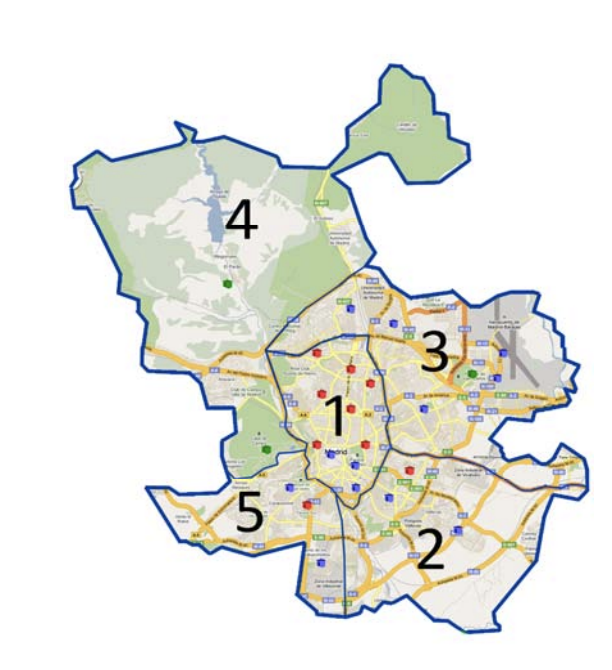
\includegraphics[width=0.4\textwidth]{zonas_madrid}
      \label{figure:stations}
  \caption{Madrid Pollution Stations and Zones.}
\end{figure} 

They are classified into 
three types: background stations, suburban stations 
and traffic stations. 

For this study, we have selected the Diaz Aguirre station.

After analysis of the $NO_2$ values, we have identified them 
as belonging to a lognormal distribution and therefore we transformed to 
the log of the values. This has 2 positive effects: the tail of a normal distribution 
is not as long as for the lognom (so we will have better quantile estimations) and 
it helps with linear models like the linear quantile regression.

The time series for this station consists of hourly
measured values of the airborne concentrations of NO2
from 01/01/2000 to 30/11/2017. These values exhibit a clear intraday 
pattern, in which the
higher values are located in two peaks around the morning
and evening (with highest average value at 19h) while the 
nightly hours (from 00h to 05h) have lower average concentrations. 
Not only are the values higher at those hours, but also
the variance is, as we can see in figure \ref{figure:variance} . 
 
\begin{figure}
  \centering
      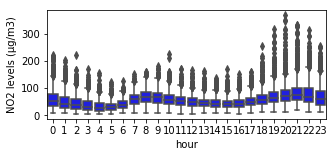
\includegraphics[width=0.4\textwidth]{NO2Var}
  \caption{Boxplot of NO2 per hour}
\label{figure:variance}
\end{figure}

In order to analyze the seasonality of the signal, we extract the 5 main factors 
from the Fourier Transform. Those can be seen clearly from the first 3000 components:

\begin{itemize}
  \item Every 12 hour Seasonality
  \item Yearly Seasonality
  \item Daily Seasonality
  \item Every 4 year seasonality
  \item Weekly Seasonality
\end{itemize} 

Therefore, we will create as input the output of periodic functions (cos) whose frequency is equal to the ones found 
above. This will enable the machine learning model learn the seasonality of our time series.

As with any forecast technique based on machine learning, we add previous values to improve the accuracy 
of the analysis. Based on the seasonal analysis, we see it's interesting to add a week of values. We will not 
add more to keep a reasonable number of features as input.

\subsection{$O_3$}

The Diaz Aguirre station also recorded the levels of $O_3$. As we can see in figure \ref{figure:no2vso3},
there seems to be a correlation between $NO_2$ levels and $O_3$.

\begin{figure}
  \centering
  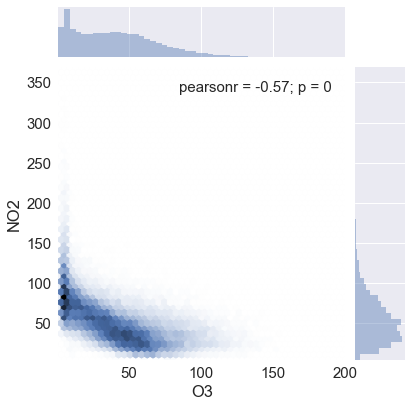
\includegraphics[width=0.4\textwidth]{no2vso3}
  \label{figure:no2vso3}
  \caption{Levels of $O_3$ vs levels os $NO_2$}
\end{figure}

We will also add lagged values of $O_3$ to our models.

\subsection{ECMWF numerical pollution prediction}
\label{sec:ecmwf-numer-poll}

The European Centre for Medium-Range Weather Forecasts implements the Copernicus Atmosphere Monitoring Service.
This service provides CAMS delivers a saily production of near-real-time European air quality analyses and forecasts 
with a multi-model ensemble system. 
As you can see in the figure \ref{figure:camspoints}, the scope of the forecast is european and does not have the needed granularity to forecast 
the levels of NO2 in a station.

\begin{figure}
  \centering
  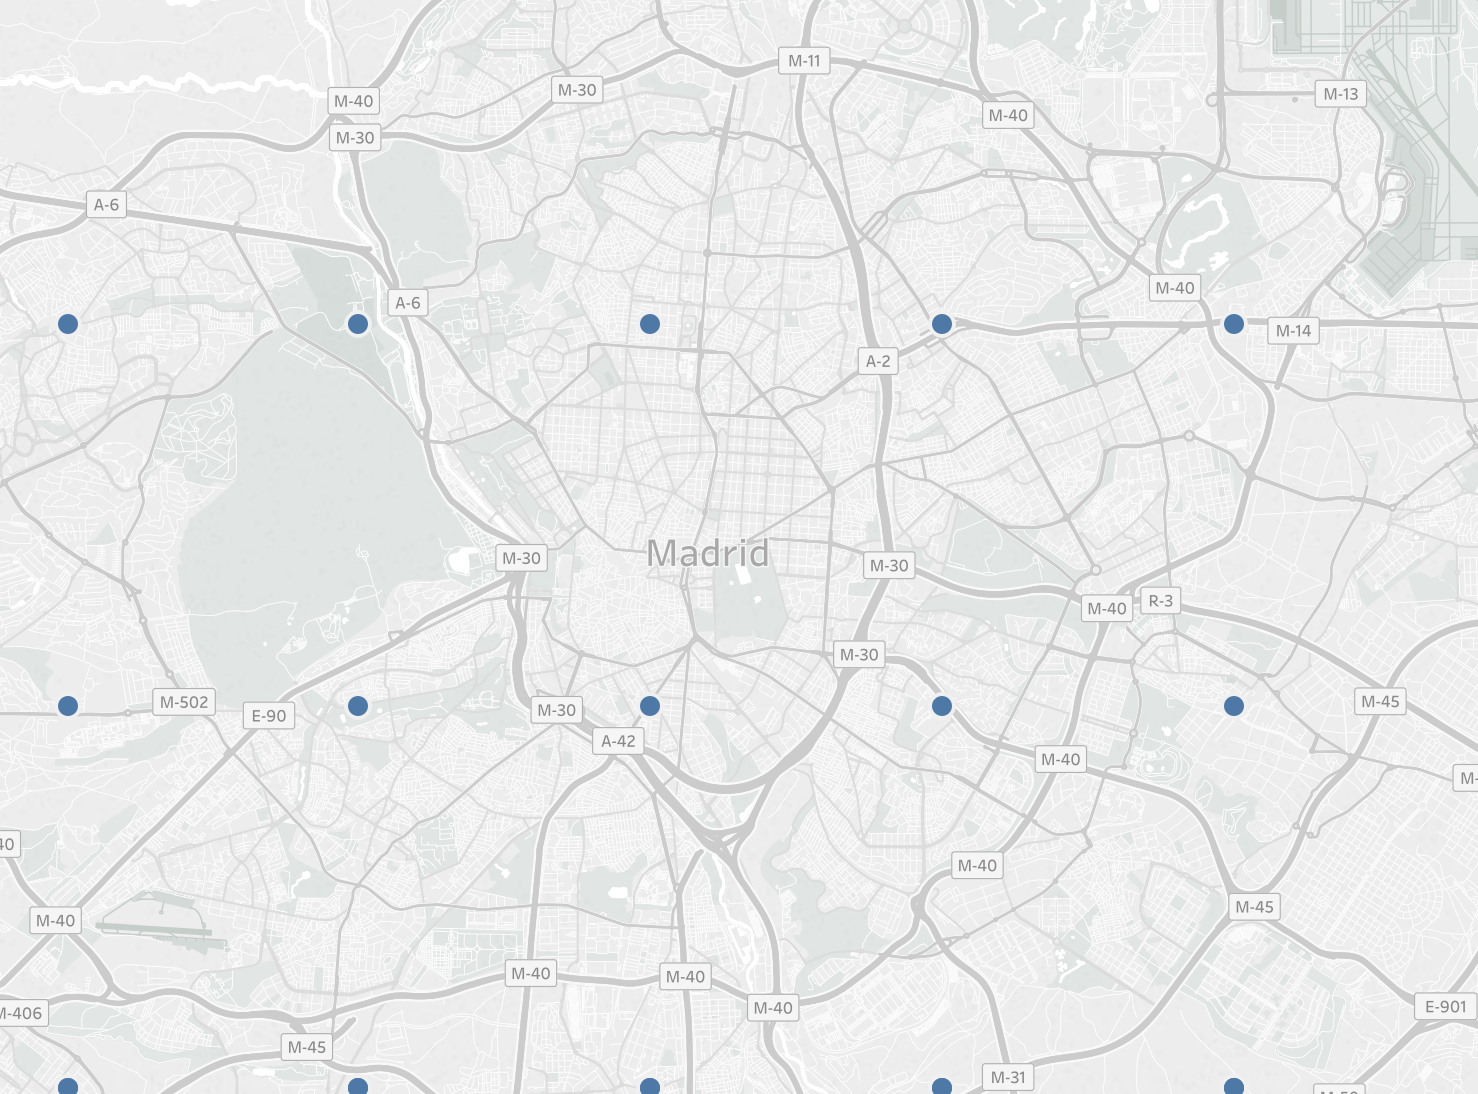
\includegraphics[width=0.4\textwidth]{camspoints}
  \label{figure:camspoints}
  \caption{Location of the points with predicted pollution from CAMS.}
\end{figure}

\subsection{Calendar Variables}
\label{sec:cal_data}

As $NO_2$ levels seem to be linked to human activity, we will also flag the hours 
belonging to a specific type of day. Days could be classified as:
-\begin{itemize}
  \item Bank holidays
  \item Heavy traffic day (for example, return from holidays)
  \item School holidays
\end{itemize} 

We will create 2 variables: one which indicates the day has a positive effect on pollution and 
another one for negative effect. We use a linear regression to predict the NO2 value only from the calendar variables.
As we can see in the figure \ref{figure:fourier}, some variables have a positive effect and others a negative effect, based on the
sign of the coefficient applied to that feature:

\begin{figure}
  \centering
  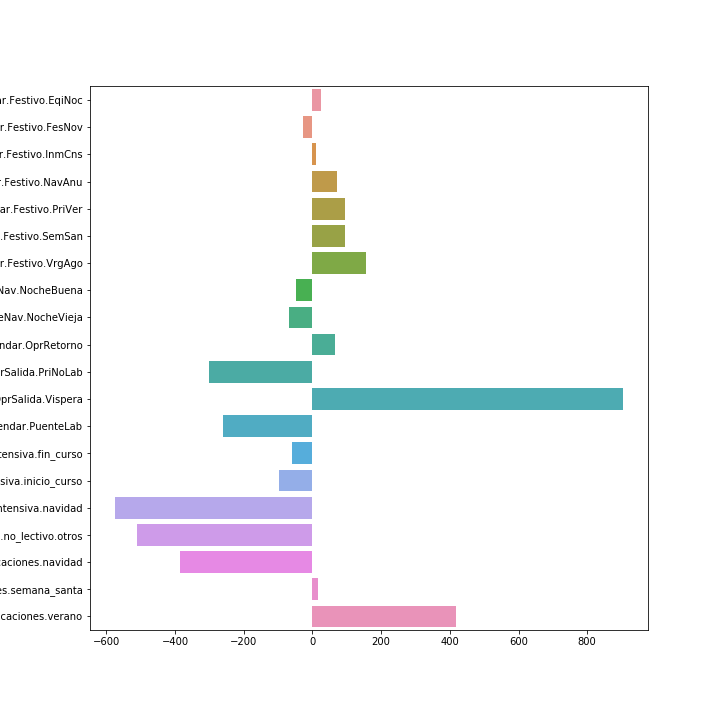
\includegraphics[width=0.4\textwidth]{calweights}
  \caption{Weights of the calendar variables.}
  \label{figure:fourier}
\end{figure}

Then we will replace the calendar variables with 2 new variables as the sum of the positive 
features and the sum of the negative features respectively.

\subsection{Experimental Design}
\label{sec:experimental-design}

First, we aligned all the hourly time series: $NO_2$, $O_3$, ECMWF in the same table 
and added the lagged values, a seasonal time series with the main periods of the $NO_2$ time series
and the calendar variables as described in section \ref{sec:cal_data}.

Once all this data is added, we will train the following probabilistic 
models:
\begin{itemize}
  \item $k$ Nearest Neighbors
  \item Quantile Random Forest
  \item Quantile XG Boost
  \item Probabilistic Xarima
\end{itemize} 

The figure \ref{figure:dataflow} shows the data flow in the experimental design.  

\begin{figure}
  \centering
  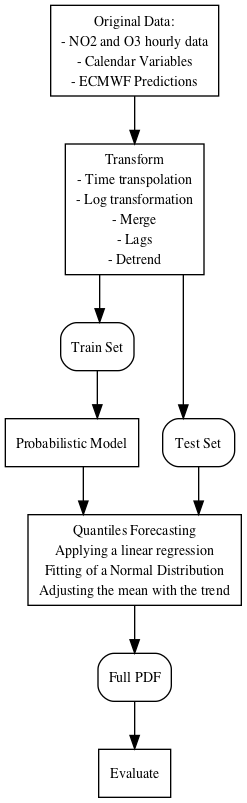
\includegraphics[width=0.2\textwidth]{diagrams/flow}
  \caption{Data flow of the experiments}
  \label{figure:dataflow}
\end{figure}

The section \ref{sec:models} provides more information on the probabilistic models.

We will train the models with data prior to 2017 and we will test our 
models with 2017 data. We will always test with 
predictions done at 10:00, as this is the time the 
forecast will be done and the alert will be decided 
or not.

After forecasting the quantiles, we will fit those quantiles in a normal distribution.
We have a low number of percentiles and we would like to get at least 100 percentiles.
Fitting a normal distribution to those percentiles and then generating the 
percentiles for that fitted distribution can generate much more percentiles 
than the ones we originally had.
Also as we do not have enough samples to estimate the upper tail of the distribution, 
we believe
fitting the distribution corrects for that and improves estimation for higher values.

We will evaluate the 50 percentile through the 
RMSE, MAE, Bias and Corr 
and the whole forecasted CDF through the CRPS. We will perform
this evaluation for each of the horizons.


\subsection{Probabilistic Models}
\label{sec:models}

We will compare the following probabilistic models:
\begin{itemize}
  \item Quantile Random Forest
  \item $k$ Nearest Neighbors
  \item Linear Quantile regression
  \item Quantile Gradient Boosting
  \item Arima
\end{itemize}

\subsubsection{Quantile Random Forest}

Quantile random forests create probabilistic predictions out of 
the original observations. It works like the usual random forest, 
except in each tree,
leafs do not contain a single value as a prediction but the target observations 
from the training set 
belonging to that leaf (see figure \ref{figure:qrandom}) . 

Then predictions are calculated by selecting the leafs in each tree
corresponding to the input features and combining the weighted 
histograms in each tree out of the target observations in those leafs. 
For more information refer to 
\cite{quantregforests}.

We decided to train a linear regressor
which predicts the $NO_2$ values from the original features and the 50th quantile, 
and then apply this linear regression 
to all the predicted quantiles. 

\begin{figure}
  \centering
  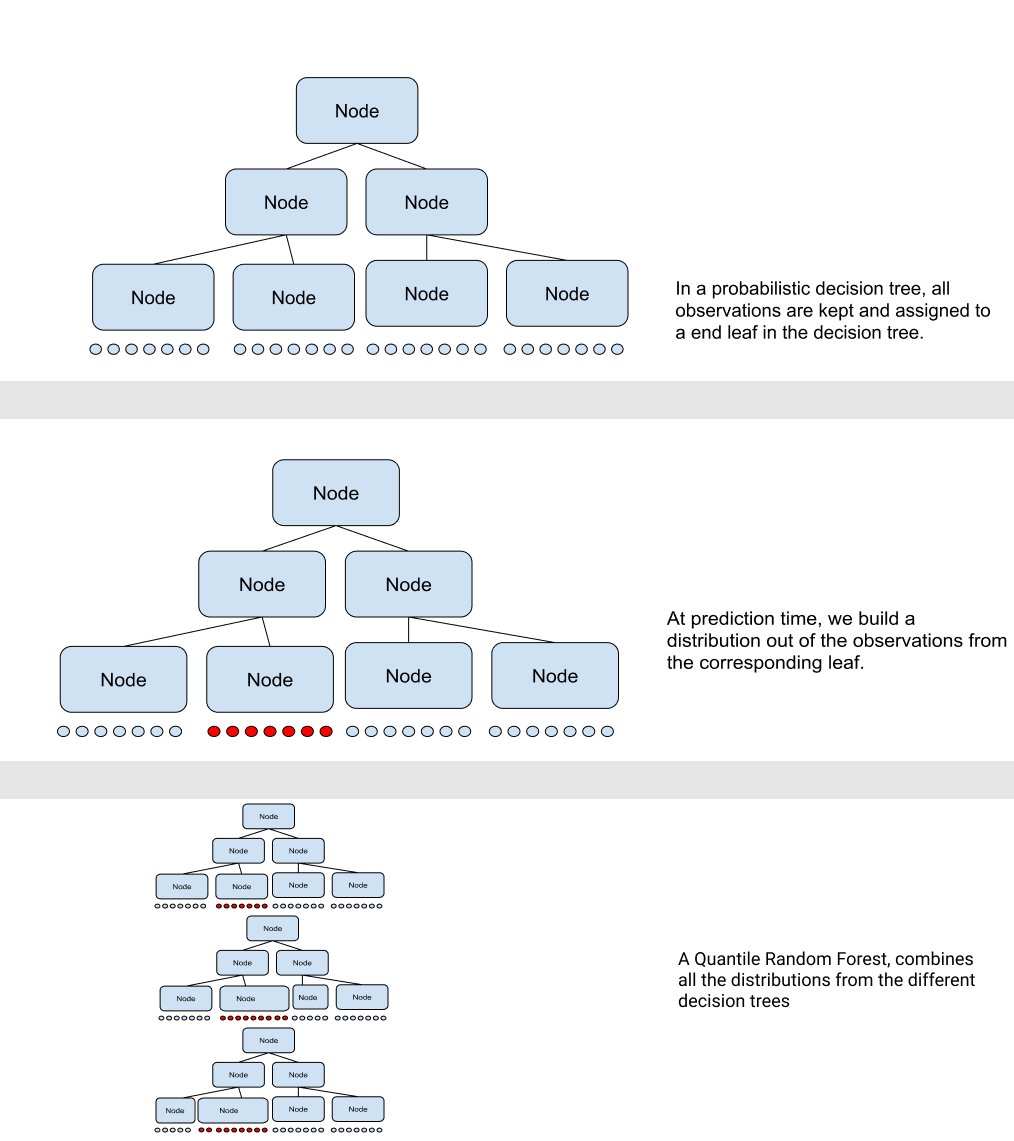
\includegraphics[width=0.4\textwidth]{quantile_random_forest}
  \caption{Random Forest Weights on observations based on trained trees}
  \label{figure:qrandom}
\end{figure}

\subsubsection{$k$ Nearest Neighbors}

We will use the probabilistic $k$ nearest neighbors algorithm as described in  
\cite{quantileknnmangalova}. 
This algorithm is based on the standard $k$ nearest neighbor, 
where instead of calculating the mean of 
the targets of the
$k$ nearest points to the input, it builds a distribution 
from those neighbors.

We found the best $k$ to be 50 after testing several values of $k$ and calculating 
the rmse for a simple regression.

We also trained a linear regressor from the original features and the 50th quantile, 
and applied it to all the predicted quantiles. 

\subsubsection{Linear Quantile regression}

We can apply linear regression with a modified cost function in order to 
predict the quantiles of the target (for a detailed discussion of 
quantile regression, refer to \cite{koenker_quantile_2005}). 

Given a 
set of vectors $(x_i, y_i)$, in point forecasting we are usually 
interested in what prediction $\hat y(x) = \alpha_0 + \alpha_1 x$
minimizes the mean squared error,
\begin{equation}
  \label{eq:1}
  E = \frac{1}{n} \sum^n_i \epsilon_i =
  \frac{1}{n} \sum^n_i [ y_i - (\alpha_0 + \alpha_1 x) ]^2.
\end{equation}
This prediction is the conditional sample mean of $y$ given $x$% , that
% is, $\hat y(x) = \hat\alpha_0 + \hat\alpha_1 x$
, or the location of the conditional distribution. But we could be
interested in estimating the conditional median (i.e., the 0.5
quantile) instead of the mean, in which case we should find the
prediction $\hat y(x)$ which minimizes the mean absolute error,
\begin{equation}
  \label{eq:2}
  E = \frac{1}{n} \sum^n_i \epsilon_i =
  \frac{1}{n} \sum^n_i | y_i - (\alpha_0 + \alpha_1 x) |.
\end{equation}
The fact is that, apart from the 0.5 quantile, it is possible to
estimate any other given quantile $\tau$. In that case, instead of
(\ref{eq:2}), we could minimize
\begin{equation}
  \label{eq:3}
E= \frac{1}{n} \sum^n_i f( y_i - (\alpha_0 + \alpha_1 x))
\end{equation}
where
\begin{equation}
  \label{eq:4}
  f(y-q) = \left\{ 
\begin{array}{l l}
\tau (y-q) & \quad \mbox{if $y \ge q$}\\
(1-\tau) (q-y) & \quad \mbox{if $y < q$}\\
\end{array} \right.,
\end{equation}
with $\tau \in (0,1)$. Equation (\ref{eq:3}) represents the
median when $\tau=0.5$ and the $\tau$-th quantile in any other case.

We will train 10 models to predict the 10 deciles of the signal. As quantiles are 
calculated separately, we have the risk of encountering quantile crossing.
We will use the simple technique as explained in \cite{cross} to solve this problem.

\subsubsection{Gradient Boosted Tree}

Tree Boosting \cite{gradientboost} is a widely used technique for machine learning 
that consist on growing trees based on the compromise 
of a cost function and a regularization function. This cost function is usually 
used to forecast 
the mean of the signal. We will modify the cost function (im a similar way as in 
the quantile linear regression) to predict the quantiles of the target. 

We will train 10 models to predict the 10 deciles of the signal and we will solve 
 quantile crossing with the technique explained in \cite{cross}. We also trained a 
 linear regressor from the original features and the 50th quantile, 
and applied it to all the predicted quantiles. 

\subsubsection{Arima}

\section{Results and discussion}
\label{sec:results}

\subsection{Reference models}
\label{sec:deterministic}

In the first experiment, we used quantile regression to compute
point-forecasts of the expected value (median) for one-day ahead
predictions of \no concentrations.

\begin{table}[tbp]
  \centering
  \label{tab:determ}
  \caption{CRPS Error for the different methods at different
    horizons (GB = Gradient Boosting,
    KNN = K Nearest Neighbor,
    LQR = Linear Quantile Regression,
    QRF = Quantile Random Forest)
    }
    \begin{tabular}{lrrrrr}
      \toprule
      method &  Arima &    GB &   KNN &   LQR &    QRF \\
      horizon &        &       &       &       &       \\
      \midrule
      1       &   6.18 &  7.27 & 11.67 &  7.23 &  7.70 \\
      12      &  13.52 & 15.84 & 21.68 & 18.13 & 17.01 \\
      13      &  12.83 & 14.53 & 20.24 & 15.44 & 15.05 \\
      14      &  11.54 & 12.05 & 19.13 & 13.24 & 13.42 \\
      20      &   7.11 &  6.79 & 14.08 &  7.36 &  7.42 \\
      37      &  13.31 & 16.28 & 19.24 & 16.71 & 16.19 \\
      45      &   9.01 &  6.96 & 12.48 &  7.90 &  8.69 \\
      55      &   6.22 & 11.50 & 17.94 & 12.63 & 13.29 \\
      \bottomrule
      \end{tabular}
  
\end{table}


Table \ref{tab:determ} shows Arima outperforms the other Machine Learning algorithms.

\subsection{Probabilistic forecasting of extreme values}
\label{sec:probabilistic}

\cite{qxgb}

\section{Conclusions}
\label{sec:concl}

\section*{References}

\bibliography{refs}

\end{document} 
%%% Local Variables:
%%% mode: latex
%%% TeX-master: t
%%% End:
